% !TEX encoding = UTF-8 Unicode
\documentclass[12pt]{article}
\usepackage{amsmath}

\usepackage{mathtools}
\usepackage{graphicx}
\usepackage{color}
\usepackage{natbib}
\usepackage{setspace}
\usepackage{amsfonts}
\usepackage{authblk}
\usepackage{url}
\usepackage{hyperref}
\hypersetup{colorlinks=true, linkcolor=black, citecolor=black, filecolor=black, urlcolor=black}

\usepackage[top=1.5in, bottom=1in, left=1in, right=1in]{geometry}
\parskip 3mm
\graphicspath{{../figs/}}


\newcommand{\jarad}[1]{\textcolor{green}{(jarad: #1)}}
\newcommand{\nacho}[1]{\textcolor{blue}{(nacho: #1)}}
\newcommand{\matt}[1]{\textcolor{red}{(matt: #1)}}

\newcommand{\I}{\mathrm{I}}


\renewcommand{\topfraction}{0.85}
\renewcommand{\bottomfraction}{0.85}
\renewcommand{\textfraction}{0.15}
\renewcommand{\floatpagefraction}{0.7}

\bibpunct{(}{)}{;}{a}{}{,} 

%-------------------------------------

\title{Bayesian Inference for a Covariance Matrix}
\author[1]{Ignacio Alvarez }
\author[1]{Jarad Niemi }
\author[2]{ Matt Simpson}

\affil[1]{Department of Statistics, Iowa State University}
\affil[2]{Department of Statistics and Department of Economics, Iowa State University}

\date{August 2014}
\pagenumbering{gobble}

\begin{document}
 
\maketitle 


\begin{abstract}
Covariance matrix estimation arises in multivariate problems including multivariate normal sampling models and regression models where random effects are jointly modeled, e.g. random-intercept, random-slope models. A Bayesian analysis of these problems requires a prior on the covariance matrix. Here we compare an inverse Wishart, scaled inverse Wishart, hierarchical inverse Wishart, and a separation strategy as possible priors for the covariance matrix. We evaluate these priors through a simulation study and application to a real data set. Generally all priors work well with the exception of the inverse Wishart when the true variance is small relative to prior mean. In this case, the posterior for the variance is biased toward larger values and the correlation is biased toward zero. This bias persists even for large sample sizes and therefore caution should be used when using the inverse Wishart prior.
\end{abstract}

%\newpage 

\section{Introduction} 

Covariance matrix estimation arises in multivariate problems including multivariate normal sampling models and regression models where random effects are jointly modeled, e.g. random-intercept, random-slope models. Bayesian estimation of a covariance matrix requires a prior for the covariance matrix . The natural conjugate prior for the multivariate normal distribution is the inverse Wishart distribution \citep{barnard2000}. Due to its conjugacy, this is the most common prior implemented in Bayesian software. However, this prior has issues: the uncertainty for all variances is controlled by a single degree of freedom parameter \citep{bda2013}, the marginal distribution for the variances has low density in a region near zero \citep{gelman2006prior}, and there is an \emph{a priori} dependence between correlations and variances \citep{visualize}. These characteristics of the prior can impact posterior inferences about the covariance matrix. 

Alternative covariance matrix priors have been proposed including the scaled inverse Wishart \citep{odomain}, a hierarchial inverse Wishart \citep{huang2013simple}, and a separation strategy \citep{barnard2000}. However \cite{visualize} states that 
\begin{quote}
Even fewer analytical results are known for these families, making it even more challenging to understand precisely the properties of such distributions. Consequently, our analytical understanding of these distributions falls short of providing us a full understanding of the inverse-Wishart distribution.
 \end{quote}
 
The objective of this study is to understand the impact of these prior choices on the posterior inference of the covariance matrix. We select some of the proposed prior models in the literature and first run a simulation study to assess the impact on posterior, then we apply each model to a real data set consisting of bird counts in national forest in the Great Lakes. 

The rest of this paper is organized as follows: Section \ref{sec:models} describes the statistical methods and the covariance prior distributions we use. Section \ref{sec:results} presents a simulation study consisting in simulate data from a multivariate normal model and make inference about the covariance matrix to compare the different priors. Section \ref{sec:birds} presents an application to bird counts in the Superior National Forest. Finally, Section \ref{sec:summary} provides the applied modeler with strategies for estimating a covariance matrix. 

\section{ Motivating example } 
In Section \ref{sec:birds} a data set consisting of bird counts in national forest in the Great Lakes is used. Wihtout describing details we use this data here to show some troubles for estimating the correlacion coeficient in a simple scenario.  

Let $y_{st}$ represent a measure of abundance of species $s$ in moment $t$, here we choose only two bird species: Veery (VEER) and White-throated Sparrow (WTSP). We are interested in the asociation of abundance between two species, captured by the correlation coefficient $\rho = cor(y_{1t}, y_{2t})$. 

Left panel of Figure \ref{motiva.rho} shows the raw data. The two scatter-plot represent two posible ways to measure species abundance: total count across locations, or using an average count acrross many locations.

In order to obtain posterior inference of the correlation coefficient, we fit a multivariate normal model with an inverse-Wishart distribution for the covariance matrix parameter. This model is described in equations \eqref{like} and \eqref{eq:wis}. 

\begin{figure}[htbp]
\centering
%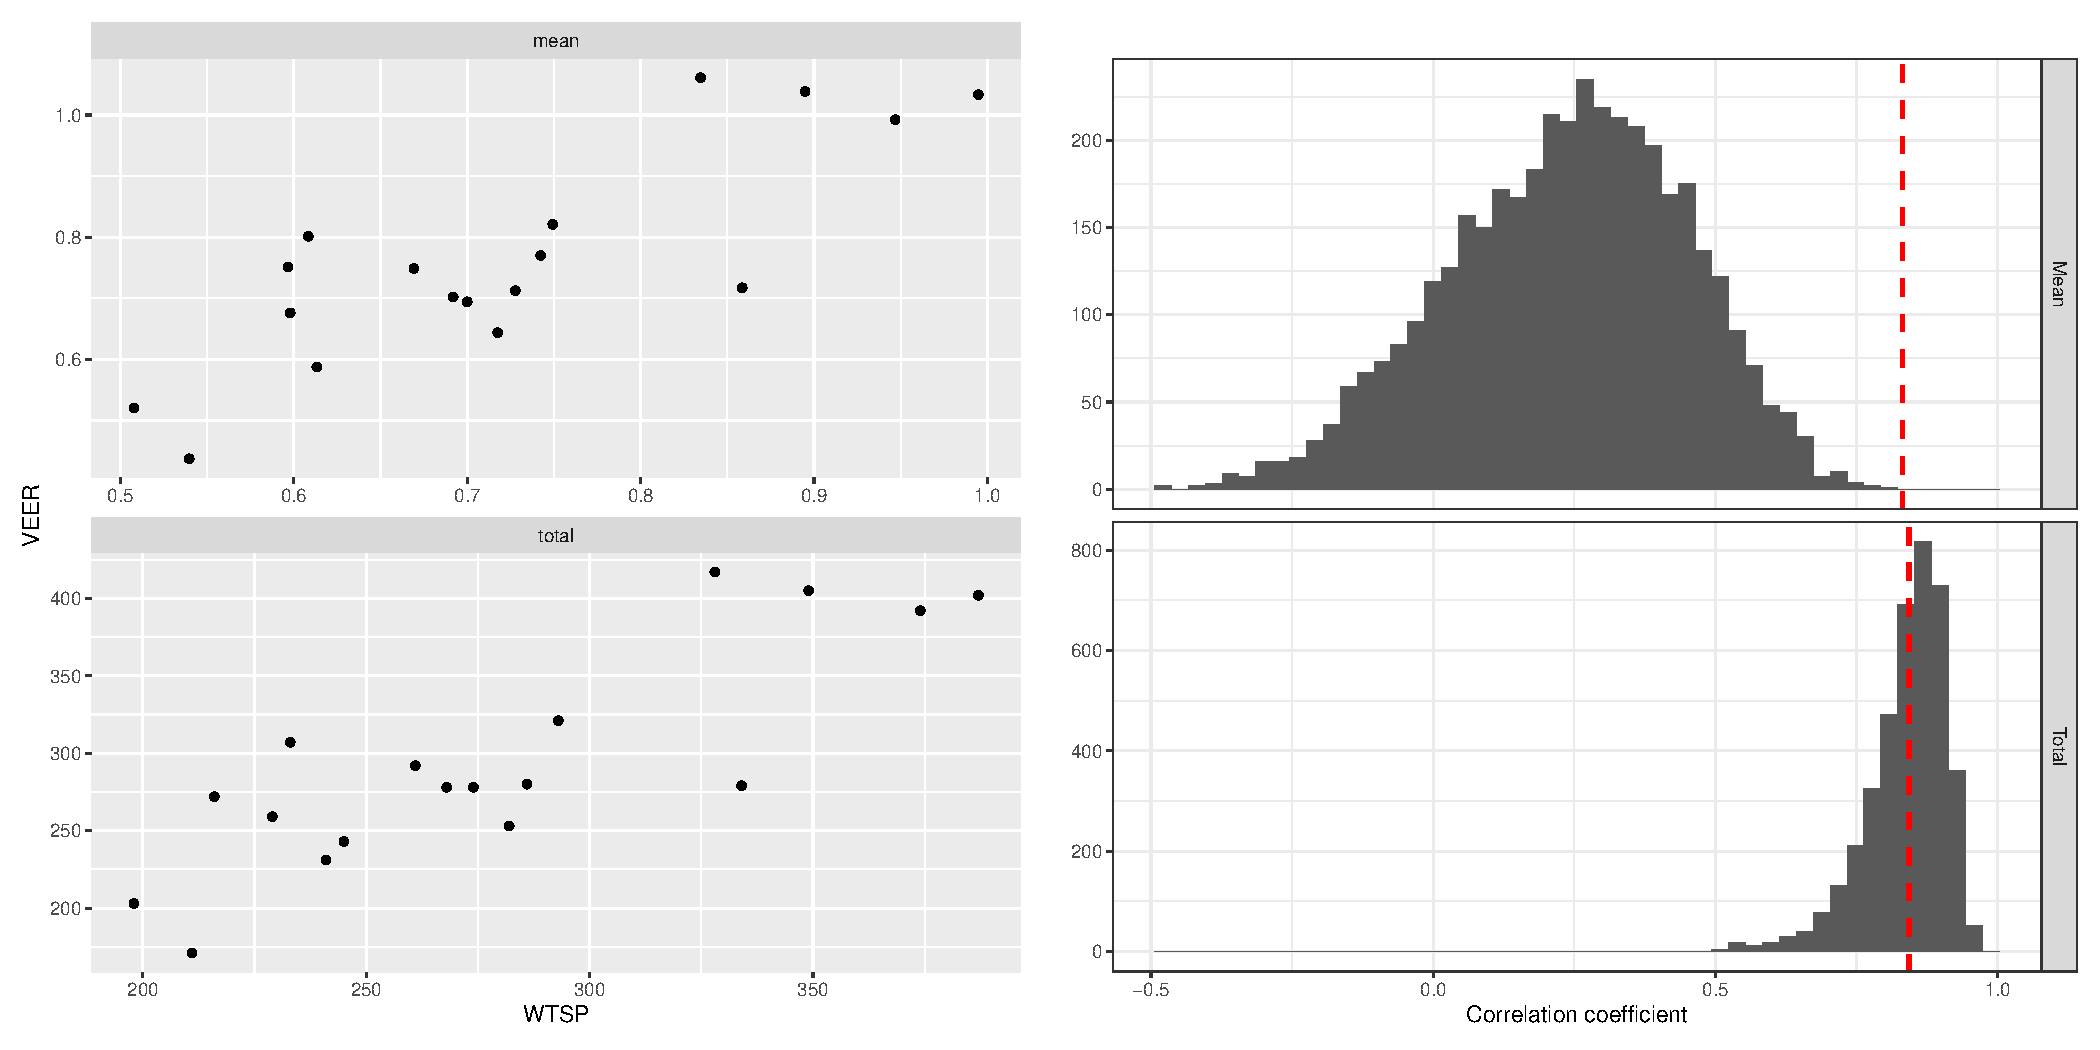
\includegraphics[trim = 0 4cm 0 3cm, clip, scale=.5]{motiva22.pdf} 
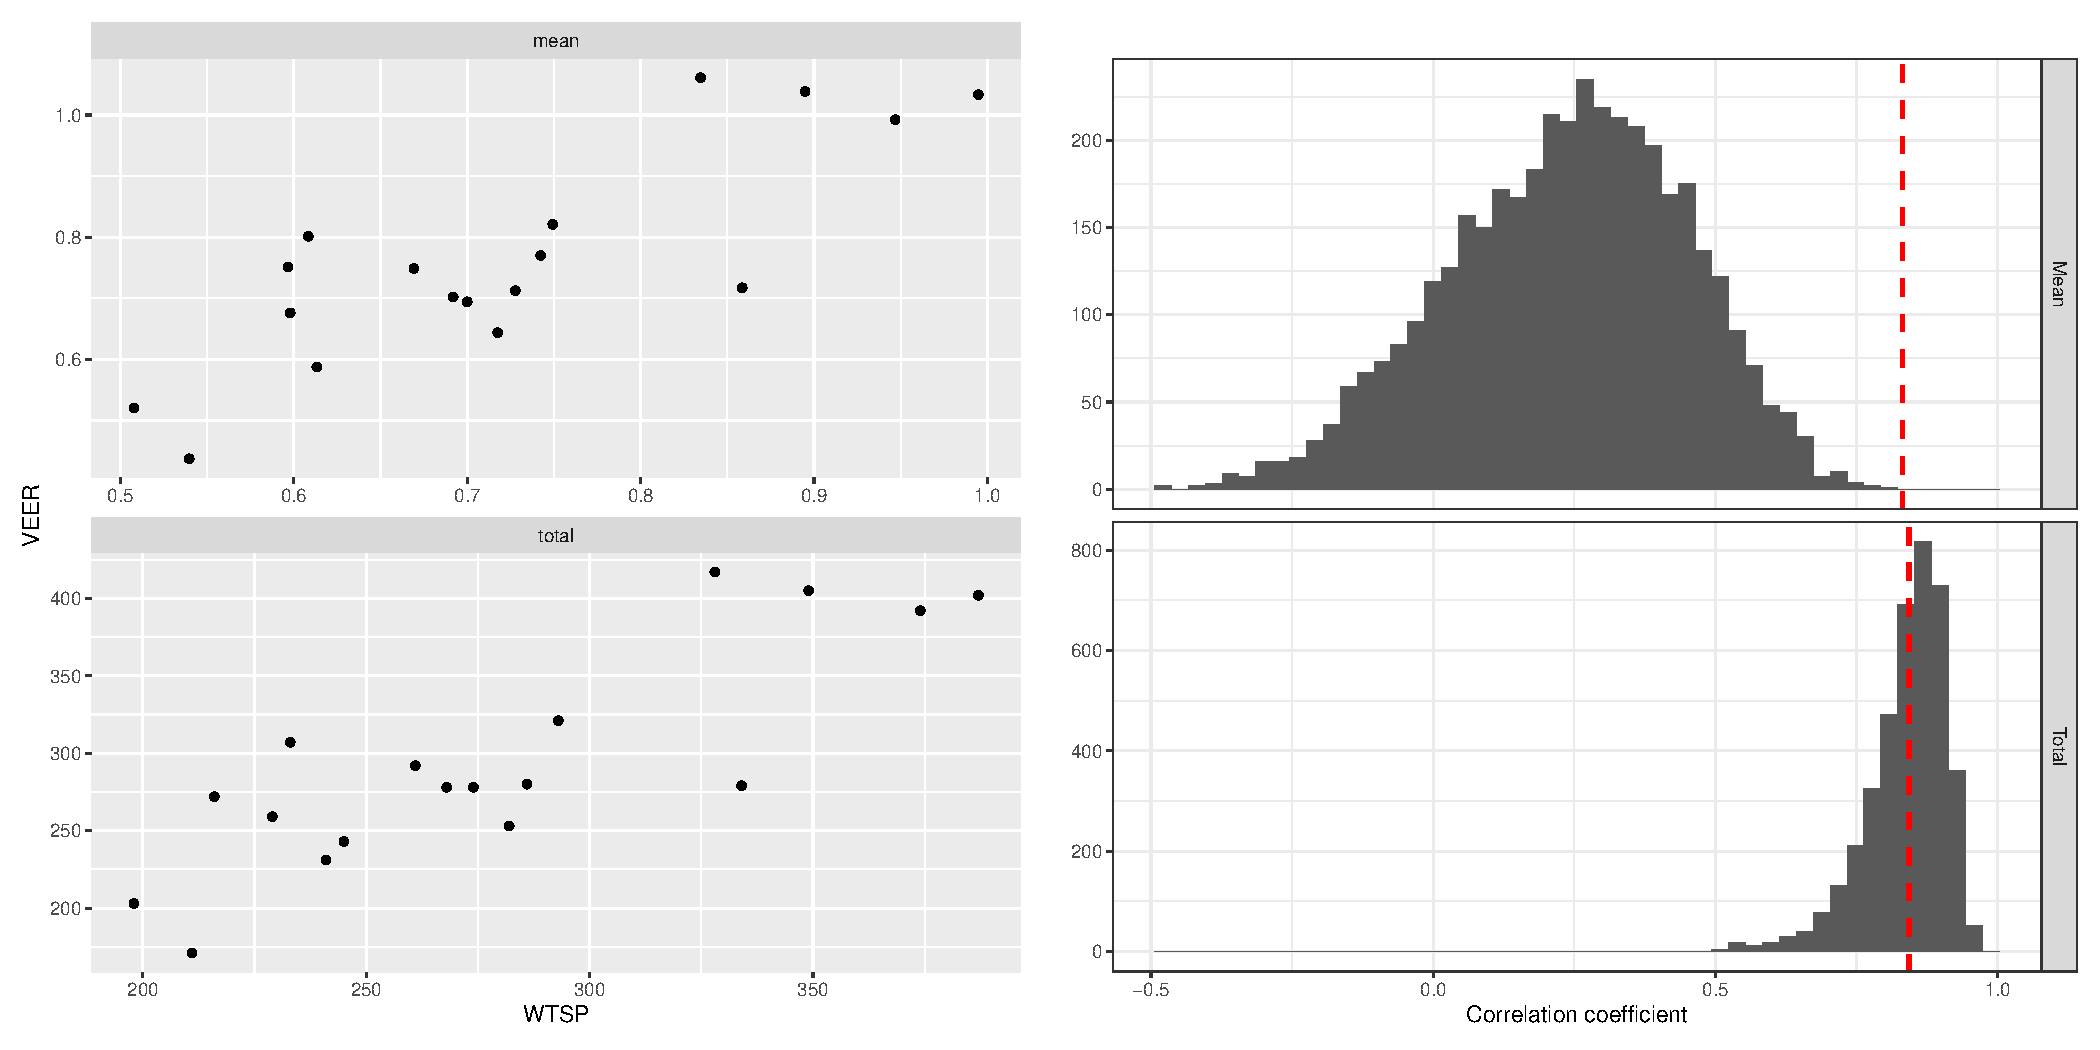
\includegraphics[scale=.5]{motiva22.pdf} 
%\vspace{-.5in}
\caption{Left panel: Scatter plot for mean abundance (top) and total abundance (bottom). Right panel: posterior distribucion of $\rho$ with mean abundance (top) and total abundance (bottom), the red dashed vertical line represent the sample correlation.  }
\label{motiva.rho} 
\end{figure}

Figure \ref{motiva.rho} shows scale of the resopnse variable might have a large impact on posterior inference and, more relevant, that using a mean response accorss locations the posterior distribution is totally off the value of the sample correlation, suggesting the prior distribution was too informative, shrinkage posterior inference towards $\rho=0$. 

\section{Statistical Models \label{sec:models} }

Consider the multivariate normal model, that is let $Y_i\in \mathbb{R}^d$ for $i=1,\ldots,n$ and assume $Y_i \stackrel{iid}{\sim} N(\mu, \Sigma)$ with $\mu\in \mathbb{R}^d$ and $\Sigma$ is a $d$-dimensional positive definite matrix.   
  \begin{equation}
 p(y\vert \mu,\Sigma) \propto |\Sigma|^{-n/2} \mbox{exp}\left\{- \frac{1}{2} \sum_{i=1}^n (y_i-\mu)^\top \Sigma^{-1} (y_i-\mu) \right\} = |\Sigma|^{-n/2}  \mbox{exp}\left\{- \frac{1}{2}  \mbox{tr}(\Sigma^{-1}S_\mu)  \right\} 
 \label{like}
 \end{equation}
The likelihood is provided in equation \eqref{like} where $y$ represents the entire data and  $S_\mu = \sum_{i=1}^n (y_i-\mu) (y_i-\mu) ^\top$. 

For this study, the primary parameter of interest is the matrix $\Sigma$ with elements $\Sigma_{ij}$. We will often refer to the standard deviations $\sigma_i$ and correlations $\rho_{ij}$ where $\sigma_i^2 = \Sigma_{ii}$ and $\Sigma_{ij} = \rho_{ij}\sigma_i\sigma_j$. 

In the following subsections, we introduce a number of covariance matrix prior classes: inverse Wishart, scaled inverse Wishart, hierarchical inverse Wishart, and a separation strategy. %One prior that is not included is the Jeffreys prior which is $p(\Sigma)\propto |\Sigma| ^ {\frac{-(d+1)}{2} } $ since this prior may lead to improper posteriors in the context of linear models \citep{gelman2006prior, SIW2008}. Finally we consider the hierarchical approach proposed by \cite{huang2013simple}, this is the most recent proposal we found for this problem. 

\subsection{Inverse Wishart prior \label{sec:iw}}

The natural conjugate prior for a covariance matrix is the inverse Wishart (IW) prior \citep{barnard2000}. 
\begin{equation} 
p(\Sigma) \propto  |\Sigma|^{-(\nu+ d +1)/2 } e^{-\frac{1}{2} tr( \Lambda \Sigma^{-1}) }
\label{eq:wis}
\end{equation}
The IW prior has density provided in equation \eqref{eq:wis} where $\Lambda\in \mathbb{R}^d$ is a positive definite $d$ dimensional matrix and $\nu$ is a scalar degrees of freedom. For a proper prior, $\nu>d-1$. The mean is $E(\Sigma) = \Sigma_0= \frac{\Lambda}{\nu - d - 1}$ for $\nu>d+1$. 

The IW prior is commonly used due to its conjugacy properties with the normal sampling model. Specifically, the full conditional for $\Sigma$ is $\Sigma \vert y,\mu \sim IW(n+\nu_0, \Lambda_0+S_\mu)$. If $\mu|\Sigma \sim N(\mu_0,\Sigma/\kappa_0)$, then the marginal posterior for $\Sigma$, $\Sigma|y$, has an IW distribution (see Sec 3.6 of \cite{bda2013}). This conjugacy allows easy incorporation into Markov chain Monte Carlo (MCMC) approaches based on Gibbs sampling.

Using an inverse Wishart prior for the covariance matrix implies a scaled inverse chi-square distribution\footnote{The scaled inverse chi-square denoted by $X \sim \mbox{inv-}\chi^2(\nu, s^2)$ has a density function given by $p(x) =  \frac{(\nu/2)^{\nu/2}} {\Gamma(\nu/2)} s^{\nu}x^{-(\nu/2 + 1)} \mbox{exp}\left\{-\nu s^2 / 2x\right\} $} for each variance $\sigma_i^2\sim \mbox{inv-}\chi^2(\nu - d + 1, \frac{\lambda_{ii}}{\nu-d+1} )$ where $\lambda_{ii}$ is the $i^{th}$ diagonal entry of $\Lambda$. If $\Lambda$ is a diagonal matrix, each correlation has marginal density as $p(\rho_{ij}) \propto (1 - \rho_{ij}^2)^{(\nu - d + 1)/2}$. A default approach for the IW prior sets $\Lambda=\I$ and $\nu=d+1$ where $\I$ is an identity matrix. A diagonal $\Lambda$ and $\nu=d+1$ results in marginal uniform distributions for all correlations. 

There are a least three problems with the IW prior. First, the uncertainty for all variance parameters is controlled by the single degree of freedom parameter and thus provides no flexibility to incorporate different amounts of prior knowledge to different variance components (see Sec 19.2 of \cite{bda2003}). Second, when $\nu>1$, the implied scaled inv-$\chi^2$ distribution on each individual variance has extremely low density in a region near zero and thus causes bias in the result posteriors for these variances \citep{gelman2006prior}.  Third, the IW prior imposes a dependency between the correlations and the variances. In particular larger variances are associated with absolute values of the correlations near 1 while small variances are associated with correlations near zero \citep{visualize}.  We illustrate the latter two problems in Section \ref{sec:results}.

%\section{Alternative priors for $\Sigma$}
%We present the alternatives to IW prior that we use in this work ordered in terms of it increasing flexibility. We start with the scaled inverse Wishart (SIW) as it is also conjugate, next we present a hierarchical inverse Wishart prior that results in  half-t priors for the variances (HIW$_{ht}$), it is not clear which of these two options is the more flexible. The last prior we describe is an example of the separation strategy (SS) proposed by \cite{barnard2000} which implies marginal uniform correlations (BMM$_{mu}$).  


\subsection{Scaled Inverse Wishart \label{sec:siw}}

An alternative to the IW prior is the scaled inverse Wishart (SIW) prior which is based on the inverse Wishart distribution but adds additional parameters for flexibility \citep{odomain}. The SIW prior defines $\Sigma \equiv \Delta Q \Delta $ where $\Delta$ is a diagonal matrix with $\Delta_{ii}=\delta_i$, then 

\begin{equation}
Q \sim  IW(\nu, \Lambda) \;\;, \;\; \log(\delta_i) \stackrel{ind} \sim N(b_i, \xi_i^2)
\label{eq:siw}
\end{equation} 

We use the notation $\Sigma \sim SIW(\nu, \Lambda, b, \xi)$ to refer to this prior.  By construction, the SIW prior implies that $\sigma_i = \delta_i \sqrt{Q_{ii}}$, and $\Sigma_{ij}=\delta_i\delta_jQ_{ij}$. Thus each standard deviation is the product of a log-normal and the square root of a scaled inv-$\chi^2$ and the correlations $\rho_{ij} = Q_{ij}/\sqrt{Q_{ii}Q_{jj}}$ have the same distribution they had under the inverse Wishart on $Q$.  

%\begin{eqnarray}
%\nonumber p(\sigma^2) &=& \int p(\delta_i, \sigma^2) d\delta_i \\
%\nonumber &\propto& \int \frac{e^{-(log(\delta_i)-b_i)^2/2\xi_i}}{\delta_i} \left(\frac{\sigma^2}{\delta^2}\right)^{-(\frac{\nu-d+1}{2}-1)} e^{- \frac{\lambda_{ii}\delta^2}{2\sigma^2} } d\delta_i \\
%\nonumber &\propto& (\sigma^2)^{-(\frac{\nu-d+1}{2}-1)} \int\delta_i^{\nu-d+2}e^{ \frac{-(log(\delta_i)-b_i)^2}{2\xi_i} - \frac{\lambda_{ii}\delta^2}{2\sigma^2}}d\delta
%\end{eqnarray}

This prior is recommended by \cite{gelmanhill}, setting $\nu=d+1$ and $\Lambda=\I$ to ensure uniform priors on the correlations as in the IW prior but now there is more flexibility on incorporating prior information about the standard deviations. %\nacho{ Gelman-Hill use $\delta \sim unif(0,100)$ which is also commented on BDA2013; O'maley used the lognormal but does not have a recommendation for $\xi$ }
%It could be the case that there is prior information for some of the variance parameters but not for all of them, then is possible to set up some the $\delta_i$ parameter with less variability to reflect this prior knowledge, which it was not possible to do with the IW strategy. Also having $Q\sim IW$ we can take advantage of the conjugate property facilitating the computational implementation of this model. 

\subsection{Hierarchical Half-t prior}

Recently, \cite{huang2013simple} proposed a hierarchical approach for the covariance matrix as shown in equation \eqref{eq:ht}. 

\begin{equation}
\Sigma \sim IW( \nu + d - 1 ,  2\nu\Lambda) \;\;,\;\;  \lambda_i  \stackrel{ind} \sim \mbox{Ga}\left(\frac{1}{2} , \frac{1}{\xi_i^2}\right) \;\; \mbox{with} \; E(\lambda_i)=\frac{\xi_i^2}{2} 
\label{eq:ht}
\end{equation} 
where $\Lambda$ is diagonal matrix with $i^{th}$ element $\lambda_i$. 

This prior implies a half $t$ distribution with $\nu$ degrees of freedom, location parameter 0, and scale parameter $\xi_i$.  The marginal distribution implied for correlations is giving by $p(\rho) \propto (1-\rho^2)^{\frac{\nu_0}{2}-1}$ then letting $\nu=2$ implies marginally uniform distribution for the correlation coefficient. We use the notation $\Sigma \sim HIW_{ht}(\nu, \xi)$ to denote this prior.

A similar approach was proposed by \cite{daniels1999} and \cite{matilde}, they use flat priors for the diagonal entries of $\Lambda$ matrix and put a prior on the degrees of freedom parameter.  An important advantage of  HIW$_{ht}$ is the implied half-t prior on the standard deviations which is recommended by \cite{gelman2006prior}.

\subsection{Separation Strategy \label{sec:ss} }

\cite{barnard2000} propose the a separation strategy (SS) where the standard deviations and correlations are modeled independently and then combined to form a prior on the covariance matrix. They decompose the covariance as $\Sigma = \Lambda R \Lambda$  where $\Lambda$ is a diagonal matrix with the $i^{th}$ element $\sigma_{i}$ and $R$ is a correlation matrix with $\rho_{ij}$ as the $i^{th}$ row and $j^{th}$ column element of $R$. 

\cite{barnard2000} constructs a correlation matrix $R$ from an inverse Wishart distribution. Specifically, let $Q\sim IW(\nu, I )$ then $R = \Delta Q \Delta$ where $\Delta$ is a diagonal matrix with $i^{th}$ diagonal element $Q_{ii}^{-1/2}$. The prior density for the correlation matrix is $p(R) \propto |R|^{-\frac{1}{2}(\nu+k+1) }  (\prod_{i=1}^k r^{ii}) ^{\frac{\nu}{2}}$, where $r^{ii}$ is the $i$th diagonal element of $R^{-1}$. They then assume a log-normal distribution for the logarithm of the standard deviations, i.e. $\log(\sigma_i) \stackrel{iid} \sim N(b_i, \xi_i)$.  We use the notation $\Sigma \sim \mbox{BMM}_{mu}(\nu,b,\xi)$ to denote this prior.

Under the BMM$_{mu}$ specification, individual correlations have the marginal density $p(\rho_{ij}) \propto (1-\rho_{ij}^2)^{\frac{\nu-d-1}{2}}$ and then setting $\nu=d+1$ lead to marginally uniformly distributed correlations which are also independent from the variances by construction. 

The main disadvantage of BMM$_{mu}$ is computational. %Losing the conjugacy property implies the full conditionals distributions may be harder to sampler from  and setting up a sampler is also hard due to the positive definitive constraint. In order to draw $R$ within the BMM$_{mu}$ strategy described in equation \eqref{eq:ss} we need to first sample a covariance matrix $Q \sim IW$ and then transform it  into a correlation. 
With more recently developed software, e.g. Stan \citep{stan2014}, this restriction is not as  detrimental since this software is not based on Gibbs sampling but instead on Hamiltonian Monte Carlo (HMC) which is a Metropolis strategy for all parameters simultaneously.  In fact, the STAN manual \citep{stanmanual2014} recommends following a separation strategy, but suggests the LKJ prior for the correlation \cite{lewandowski2009generating}. In high dimensions ($d>10$), the LKJ prior concentrates mass near zero correlations and therefore we do not use it here.

%This prior has a simple form: $p_{LKJ}(R) \propto |R|^{\eta-1}$  with $\eta > 0$. In order to get marginally uniform distributions on the individual correlations we should  set $\eta \in (0,1)$ and probably make it lower when the dimension of the covariance matrix is larger. However small values for this parameter make the LKJ sampler unstable. There is no a clear guide on how to set $\eta$. We will not use the LKJ prior in our simulations.

% \subsection{Options for applied modeling}
% 
% The IW distribution is probably the most common distribution used as covariance matrix prior. Conjugacy allows for easy implementation and it is relatively computationally inexpensive. The IW prior is already implemented in most Bayesian software, which is not true for any other alternative. Due to the prevalence of the IW prior and lack of obvious alternatives, it is important to be aware of the limitations of the IW prior but also it would be nice to have an easy solution to continue using it. 
% 
% The main problem for IW is that the inference for $\rho$ is affected by the scale of the data and in some cases posterior inferences can be severely impacted. However we could take advantage of the problem in order to get better inferences. Simply re-scaling the data before fitting the model will improve posterior inference for the correlation. This pre-scaling strategy is essentially the same as using the SIW prior except with a point mass prior on the standard deviations at the sample standard deviations.
% %This seems related to the SIW prior since here we are imposing another covariance matrix decomposition, $\Sigma = DQD$ where D is a diagonal matrix with the sample standard deviations and $Q\sim IW(\nu, \Lambda)$. So the main difference with SIW would be among $D$ and $\Delta$, i.e. the elements of D are fixed and known while the elements of $\Delta$ are log-normally distributed. \matt{This paragraph could be clearer. In addition, I'm pretty sure prescaling the data is essentially the same as using the SIW prior except with a point mass prior on the standard deviations at the sample standard deviations.}
% 
% A immediate problem with this method is that it only works when $\Sigma$ is the covariance matrix of observed data. If $\Sigma$ appears related to some random effects covariances matrix in a linear model or another parameter vector in some hierarchical model we can not scale those in order to use this correction.  Maybe one option is to fit the model with an IW prior, get an estimate for standard deviations and then re-estimate the model scaling the parameters. %\matt{Again, could be a bit clearer. Refer to scaled the data before running fitting the model with an IW prior by name - e.g. $IWsc$, which you use later in a plot.}
% 
% We will add this as another strategy to define a prior for $\Sigma$ matrix. The procedure is first scale the data so that marginally each variable has a standard deviation of 1, then use the IW prior described in Section \ref{sec:iw}. We present results for the cases in which the traditional IW approach has serious problems estimating the correlations. 

\section{Simulation study results \label{sec:results}}

In this section we carry out a simulation based analysis to assess the performance of these different covariance matrix prior. First, we simulate from each prior to study the \emph{a priori} relationship between correlations and standard deviations. Second, we simulate data from the model and analyze posterior means to determine the impact prior choice has on posterior inference. Table \ref{paramvals} presents the hyperparameter values used in both simulations study for every prior. 

We started with the default IW$(d+1,\I)$ prior which implies a marginal uniform prior on the correlations and an IG$(1,1/2)$ marginal prior for the variances. We set hyperparameters for the other three priors to imply marginal uniform priors for the correlations and prior medians on the variances to match the median of an IG$(1,1/2)$ of 0.72.    

\begin{table}[htbp]
   \centering
    \caption{ Parameter values for simulation study}
   \label{paramvals} 
   \begin{tabular}{ l|c|c}
   \hline
      Prior    &  Values for prior sampling & Values for posterior inference\\ \hline
  IW$(\nu, \Lambda)$ &   $\nu=d+1$, $\Lambda=\I$  & $\nu=d+1$, $\Lambda=\I$  \\ 
  SIW$(\nu, \Lambda, b, \xi)$  & $b=0$, $\xi_i =1$,  $\nu_0= d + 1$, $\Lambda = 0.8\I$ & $b=0$, $\xi_i =100$,  $\nu_0= d + 1$, $\Lambda = \I$ \\
  HIW$_{ht}(\nu, \xi)$    &  $\nu=2$,  $\xi_i=1.04$ & $\nu=2$,  $\xi_i= \sqrt{1000}$ \\
   BMM$_{mu}(\nu,,b,\xi)$   &  $\nu=d+1$, $b_i=\log(.72)/2$ , $\xi_i=1$ &  $\nu=d+1$, $b_i=0$ , $\xi_i=100$ \\ \hline
   \end{tabular}
 \end{table}       


\subsection{Sampling from the priors} 

Figure \ref{priorF2} shows a scatterplot with the first two standard deviations from 10,000 draws from each of the four priors. The IW prior implies a positive relationship among the standard deviations. Also large correlations values appear more predominantly when the two variances are high, while low correlations appears when variances are low. 

\begin{figure}[htbp]
\begin{center}
 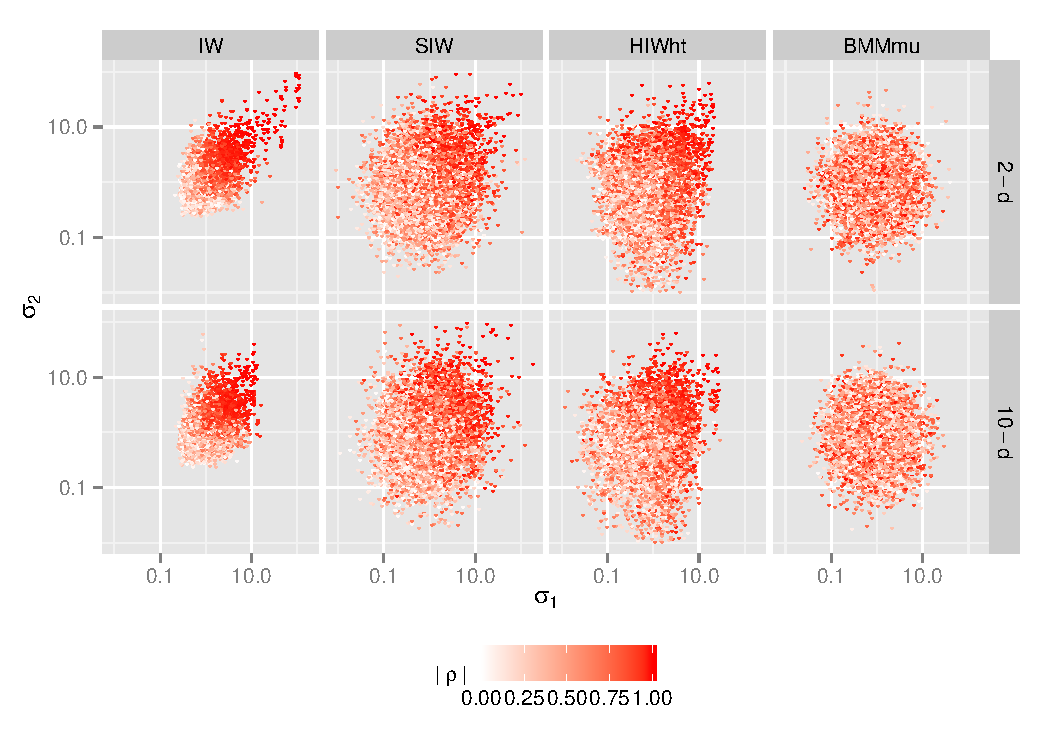
\includegraphics[width=\textwidth ]{prior_sis2.pdf} 
  \vspace{-.5in}
\caption{Samples from the prior distribution for the first two standard deviations coded by absolute value of the correlation for the four covariance matrix priors (columns) for a two- and ten-dimensional matrix (rows).}
\label{priorF2} 
\end{center}
\end{figure}

The SIW and HIW$_{ht}$ priors show a similar picture to the IW prior but the dependence is weaker. For instance, the high correlations are mostly present when standard deviations are also high, however we do see some red points for small values of the standard deviations. In contrast, the BMM$_{mu}$ prior displays draws that are independent by construction. 

%Describe a covariance matrix distribution is a hard task, \cite{visualize} propose visualization method consisting in four layers of static plots to do this. They use different scatter and contour plots plus some multivariate measures for the structural dependency in the covariance matrix. Start with two layers of marginal plots, histograms for $log(\sigma_i)$ and $\rho_{ij}$ and then scatterplots for $log(\sigma_i)$ and $\rho_{ij}$. The third layers consist in a contour of a $\Sigma$ $2\times2$ sub-matrix, which can be associated with a 50\% equiprobability ellipse from a normal distribution, this gives information about orientation and spread of the points also this layer has a 3-dimensional plot. Finally they include measures for studying multivariate relations on the matrix are the Effective Variance and Dependence statistics to be $V_e = |\Sigma|^{\frac{1}{d}}$ and $D_e=1-|R|^{\frac{1}{d}}$ respectively ($R$ is the correlation matrix associated with $\Sigma$). 
%\begin{description}
%\item[\textbf{Layer 1:}] Histograms for $log(\sigma_i)$ and $\rho_{ij}$ 
%\item[\textbf{Layer 2:}] Construct $ {d(d+1) \choose 2}  $ Scatterplots for $log(\sigma_i)$ and $\rho_{ij}$ 
%\item[\textbf{Layer 3:}] Contour and 3-dimensional plot. A $2\times2$ sub-matrix can be associated with a 50\% equiprobability ellipse from a normal distribution, this gives information about orientation and spread of the points. 
%\item[\textbf{Layer 4:}] The use two scalar statistics for study multivariate relations on the matrix. Pena and Rodriguez propose Effective Variance and Dependence statistics to be $V_e = |\Sigma|^{\frac{1}{d}}$ and $D_e=1-|R|^{\frac{1}{d}}$ respectively ($R$ is correlation matrix associated with $\Sigma$). 
%\end{description}
%We explore the priors simulations using similar plots than what \cite{visualize} propose, however we do not apply its visualization method exactly.  


%\begin{figure}[htbp]
%\begin{center}
% \includegraphics[width=\textwidth ]{priorsim2d} 
% \vspace{-.5in}
%\caption{Scatterplot of prior samples, correlation coefficient and standard deviation of the first component (on $\mbox{log}_{10}$ scale). Column panels represent each covariance prior and the row panels are the dimension of the data.  \label{priorF1}}
%\end{center}
%\end{figure}
%Figure \ref{priorF1} shows scatter plot of 10000 draws of each of the four priors to observe the relationship between correlation and standard deviation implicit in each of these priors. 
 % We can see the relationship between $\rho_{12}$ and $\sigma_1$ with the IW prior, for values of the standard deviation close to 1 the correlation can vary freely across -1 to 1, however when $\sigma_1$ get small the range for $\rho$ start to shrink towards zero and when the standard deviation is high the IW prior seem to pull the correlation to big absolute values. The SIW and HIW$_{ht}$ priors alleviate this issue to some extent we can still see some relationship, for large values of the standard deviation each prior put less weight on correlation values close to zero.  As expected BMM$_{mu}$ prior is different, here there is not a relation among $\sigma_1$ and $\rho$, which is reasonable if we recall that those parameters are sampled independently within this strategy. 



\subsection{Impact on posterior} 

The prior relationship between standard deviations and correlations presented in the previous section may or may not be an issue depending on how much this relationship impacts the posterior. To concentrate on estimation of the covariance matrix and its constitutive components, we simulate mean-zero, normally distributed data in two and ten dimensions with equal variances in all dimensions. A similar approach is taken by  \cite{daniels1999} and \cite{matilde} in their simulations.

We study the sensitivity of correlation and standard deviation point estimates to the choice of the covariance matrix prior. Table \ref{scen} shows the sample size, standard deviation, and correlations used in the simulation study. We conducted a full factorial experiment with 5 replicates at each combination.

% The bivariate case $d=2$ data came from the following model 
% \begin{equation}
% \begin{pmatrix}  Y_1 \\ Y_2 \end{pmatrix} \sim 
% N\left( \begin{pmatrix}  0 \\ 0 \end{pmatrix}, \begin{pmatrix}  \sigma_{1}^2 & \rho\sigma_{1}\sigma_{2} \\ \rho\sigma_{1}\sigma_{2} & \sigma_{2}^2 \end{pmatrix} \right)
% \label{modsim}
% \end{equation}  

\begin{table}[htbp]
   \centering
   \caption{Simulation scenarios. Specific values used in simulations for each parameter. \label{scen}} 
     \begin{tabular}{lcc} \hline
          &  Bivariate    & Ten-dimensional  \\ \hline
      Sample size   ($n$)   & 10, 50, 250   &  10, 50  \\
      Standard deviation ($\sigma$)  & 0.01, 0.1, 1, 10, 100 & 0.1, 1, 100 \\
      Correlation ($\rho$)   &  0, 0,25, 0.5, 0.75, 0.99  &  0, 0.99 \\ \hline
   \end{tabular}
\end{table}

%Another aspect that will directly affect the estimation results is the sample size, here we consider 3 different values, from a small sample to a fairly big sample, $n=250$ would be consider as a big sample size in the bivariate case where there are only 3 parameters to estimate, in ten dimensions the number of parameter to estimate increase up to 55 but also there are more data since now each observation corresponds to ten observed values. \matt{most of the information in this paragraph seems unnecessary}
To reduce Monte Carlo variability in the simulations, data were simulated for $\sigma=1$ and then rescaled to get obtain simulations with the other variances. For instance, five replicate data sets that consists of ten observations from a bivariate independent standard normal, i.e. $n=10$, $d=2$ $\rho=0$ and $\sigma=1$, were simulated. Each simulated value is multiplied by 0.01 (or 0.1, 10, and 100) to obtain data sets with standard deviation approximately 0.01 (or 0.1, 10, and 100).

The models are estimated using Stan software (\cite{stan2014}) which uses a HMC algorithm to construct posterior samples with the No U-turn sampler (NUTS, \cite{hoffman2011no}) strategy. Default initial values were used. Model convergence is monitored using the potential scale reduction factor \citep{bda2003}.
Initially, 3 chains with 1000 iterations after burn-in is used for every model. Whenever the reduction factor is bigger than 1.1 a longer model with 2000 iterations per chain after burn-in period is estimated.  

\subsubsection{Inference for Correlation coefficient}

For inference, the true sampling model is assumed and the covariance matrix priors shown in Table \ref{paramvals} were assumed with the parameter values for posterior inference column. Only the bivariate results are shown here but the ten-dimensional results are similar.

\begin{figure}[hbtp]
\centering
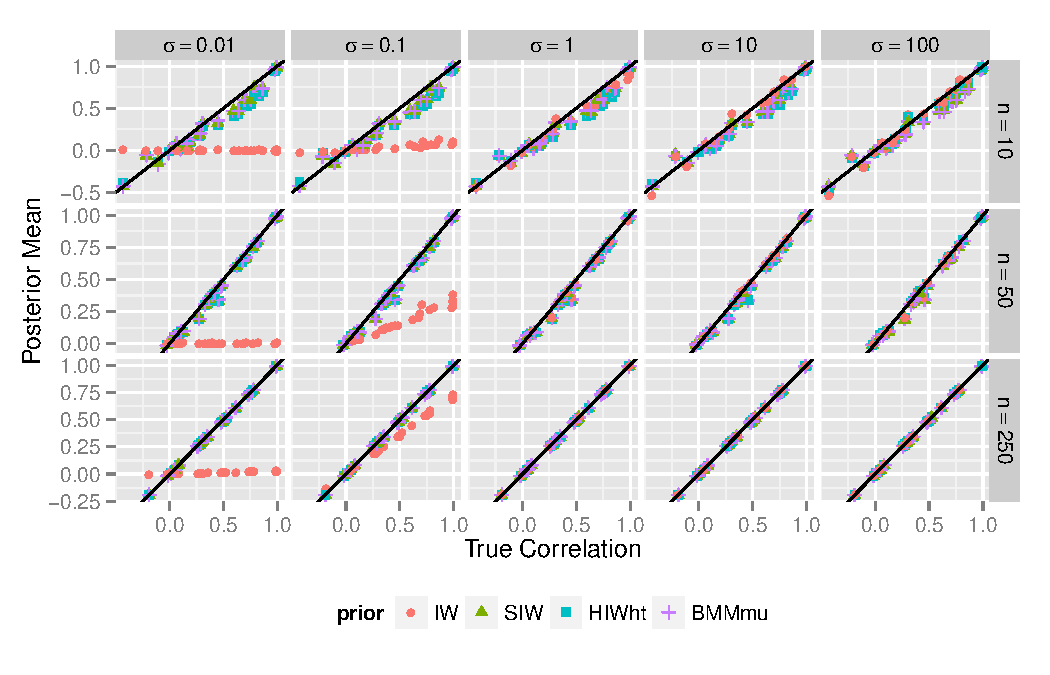
\includegraphics[width=\textwidth] {fig_rho_d2.pdf} 
\vspace{-.5in}
\caption{Posterior mean of the correlation (vertical axis) versus jittered true correlations for the range of true standard deviations (columns) and sample sizes (rows) using the four covariance matrix priors.}
\label{rhod2}
\end{figure}

Figure \ref{rhod2} shows the estimated posterior means compared with the values used in the simulation. This figure shows that when the standard deviation is small the IW prior heavily shrinks the posterior correlation towards 0 even if the true correlation is close to 1. This bias is attenuated as the sample size increases, but is still remarkably large with 250 observations when the standard deviation is around 0.01. 

All other priors appear to recover the true correlation with a slight bias toward zero for small sample sizes.
%Posterior means for all the rest of priors in the bivariate case  do not show the bias effect for the small variance case, mostly all estimates are near the true value and the variability gets smaller when the sample size increase.  The biggest issues with these estimates is the case where no correlation and the sample size is small but does not seem to be affected by the variance.  With only 10 data points we could expect lot of variability in the correlation estimates,Figures \ref{rhod10}  shows the results for the 10-dimensional case. Again we can see the bias in the posterior mean when the variance is small and we use IW prior, actually the bias get bigger than the bivariate case, here for a true correlation value of 0.99 the posterior means using IW prior are close to 0 with  $n=10$ and $\sigma=0.01$. Also in ten dimensions is more clear that when the variance gets bigger the $\rho$ posterior mean increase its variability when true correlation values are zero. Figure \ref{d2d10} in the appendix shows the posterior means comparison across dimension, basically we can see that the inference for the correlation among the first two components is almost the same when those components represent the complete data set and when are the first two variables  in a ten dimensional vector. 
% \begin{figure}[htbp]
%    \centering
%    \includegraphics[width=\textwidth]{cilength} % requires the graphicx package
%     \vspace{-.5in}
%    \caption{Length for a 95\% credible interval for $\rho$. Each panel represent a standard deviation value,  color represent the covariance prior, sample size is $n=10$ in every case.  \label{cilength}}
% \end{figure}
% 
% We compute the length of a 95\% credible interval and results are shown in Figure \ref{cilength}. The parametric space for the correlation is bounded, so a credible interval centered on 0 is more likely to be longer than if were close to 1. We use the Fisher transformation\footnote{ Fisher transformation for the correlation coefficient is defined as $z = \mbox{log} \left( \frac{1 + \rho}{1 - \rho} \right)$ where $\rho$ is the correlation. } for the correlation coefficient to map its parametric space onto the whole real line, and then get fair comparison of the length of the credible intervals.
% 
% Credible interval length is highly affected by sample size getting smaller when sample size increase, obviously this is not surprising.  Since for sample size of $n=50$ and $n=250$ it no difference among any of the prior so these cases are not shown in the figure. For the small sample size case, credible intervals are wider on high correlations for every prior except IW which is extremely biased


%\subsubsection{Inference for standard deviation}

Figure \ref{devF1} shows a scatterplot of the standard deviation posterior mean against the values used in the simulation. The figure shows that the IW prior overestimates the standard deviation for true values of the standard deviation that are small.  This bias is attenuated somewhat as sample size increase, but when the true standard deviation is 0.01 the bias is still quite large even with 250 observations. 

\begin{figure}[htbp]
\centering
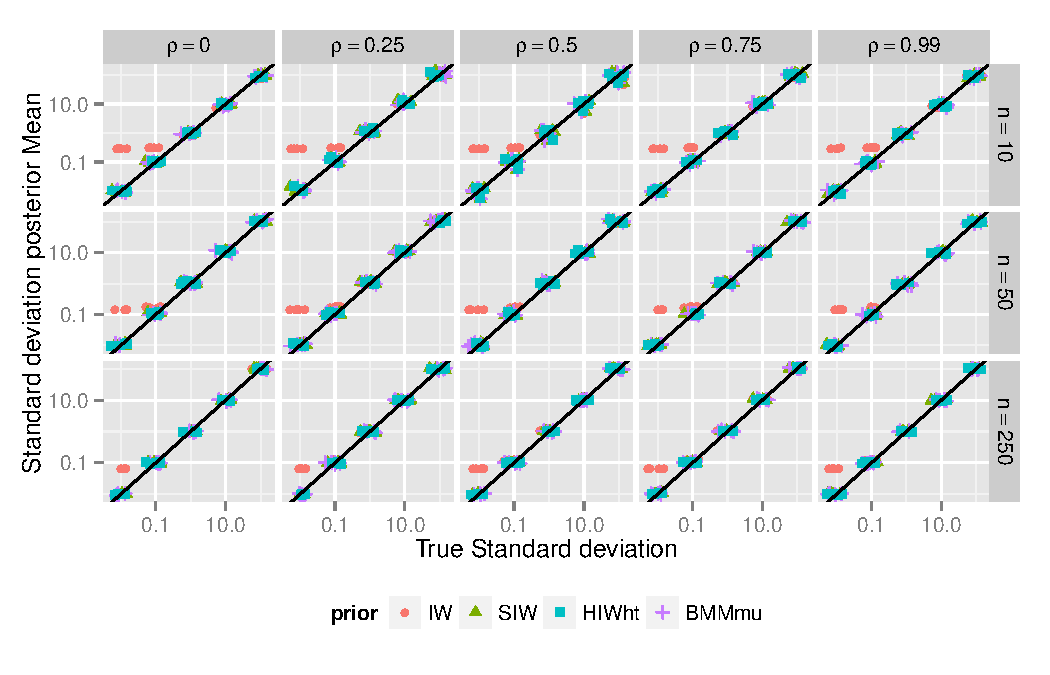
\includegraphics[width=\textwidth]{fig_s1_d2.pdf} 
\vspace{-.5in}
\caption{Posterior mean of the first standard deviation (vertical axis) versus jittered true standard deviations for the range of true correlations (columns) and sample sizes (rows) using the four covariance matrix priors.}
\label{devF1} 
\end{figure}

All other priors appear to have no difficulty in accurately estimating the standard deviation.  

% \begin{figure}[htbp]
%    \centering
%    \includegraphics[width=\textwidth]{cilength_s1}
%     \vspace{-.5in}
%    \caption{Length for a 95\% credible interval for $\sigma_1$ with sample size $n=10$. Each panel represent a correlation value,  color and shape represent the covariance prior. \label{devF3} }
% \end{figure}
% %Figure \ref{devF2} shows the standard deviation results for simulation study on the ten dimensional case, results are quite similar compare with the two dimension data sets case, IW prior shows a high bias in estimating small standard deviations for any value os the correlation.  
% Figure \ref{devF3} presents credible interval length for $\sigma_1$ for every model we fit. Overall the length of the interval increases linearly with the scale of the true value for $\sigma$. The only cases that do not follow this is when there is a small variability in the data set and IW prior is used. When the estimate from an IW prior is really biased the credible interval is really wide covering the true value. 
%There are some differences among the inference results for correlations and standard deviations. In both cases IW prior presents biased results for some scenarios, however in correlations this occurs only when the variably is low and correlation high, the bias in small variance estimation appears to be independent from the correlation true value.  The length for credible intervals in IW prior, shows the biased estimate of the correlation has no too much uncertainty while this uncertainty is really big for the biased values in the standard deviations. 

We also assessed the posterior means for the covariance, the product of the correlation and two standard deviations, and found no evidence of bias for any of the priors \citep{CCalvarez}. For the IW prior, the lack of bias here appears to be due to the marginal prior for the covariance, which does not have a closed form, having heavy tails. 

Under these simulation conditions, we find the IW prior to have no bias in estimating the covariance, to be biased toward large values for small variances, and to be biased toward zero for correlations when the variance is small. Intuitively, the heavy tailed-ness in the marginal prior for the covariance results in robust estimation for the covariance, but the lack of prior mass near zero in the marginal prior for the variance results in an upward bias. Since a correlation is a covariance divided by two standard deviations, the only way to reconcile these results is to have a corresponding bias in the correlation toward zero.

% The combination of the results presented in Figures \ref{rhod2} and \ref{devF1}  suggest that in the IW prior, the overestimation of the standard deviation is causing the underestimation for the correlation coefficient. To explore this explanation we should consider the estimates for the individual covariance terms. 
% 
% Figure \ref{devCov} presents the posterior means results for the covariance parameter $\sigma_{12}=\rho\sigma_1\sigma_2$. Each panel is a scatter-plot of the posterior mean of $\sigma_{12}$ against its true value for a specific value of standard deviation and sample size. As we are simulating scenarios where $\sigma_1 = \sigma_2$ within each panel different values of covariance also represent different values for correlation. 
% 
% We can see there is no bias in the covariance estimation for any of the priors. Particularly for IW the uncertainty is higher than for the others priors but there seems to be no clear bias in the estimate. 
% \begin{figure}[htbp]
%    \centering
%    \includegraphics[width=\textwidth]{fig_cov_d2} 
%     \vspace{-.5in}
%    \caption{Bivariate data results. Scatterplot of posterior mean for $\sigma_{12}=\rho\sigma_1\sigma_2$  against its true value used in simulation. Each panel is a combination of standard deviation (columns) and sample size (rows),  color and shape of the points represent the covariance prior. \label{devCov} %\matt{Similar comment here as for Figure 2, though I don't know how to fix it.}
% }
% \end{figure}

% \subsection{Inverse Wishart on pre-scaled data}
% 
% Based on these results, we suggest avoiding the conjugate IW prior, but due to software limitations this may not always be possible. In cases when the use of an IW prior is unavoidable and a posterior mean results in an estimated variance that is small, say below 1, the results for both the standard deviation and correlation should questioned. 
% 
% If the quantity of interest is the correlation, then an approach that can be used is to pre-scale the data so that the empirical variance is one and fit the model using the IW prior and the correlations will be estimated without bias. 
% 
% Figure \ref{sciw} illustrates this solution. We can see the bias for large correlation values is no longer a problem. This plot looks similar to the results from the alternative priors studied here shown in Figure \ref{rhod2}, although with increased variability amongst the point estimates. 
% 
% \begin{figure}[htbp]
% \centering
% \includegraphics[width=\textwidth]{scIW} % requires the graphicx package
% \vspace{-.5in}
% \caption{Posterior mean for the correlation (vertical axis) versus the true correlation (horizontal axis) for different true standard deviations (columns) and sample sizes (rows) when the IW prior is applied to data scaled to have a variance of one.}
% \label{sciw}
% \end{figure}



\section{Bird counts in the Superior National Forest \label{sec:birds}}

The Natural Resources Research Institute conducts a long-term monitoring program in Superior National Forest to track regional avian population trends. The specific data set which it is used in this manuscript consist of the yearly bird counts for the 10 most abundant species from 1995 to 2013. 
% A first look of the data is shown on Figure \ref{figtr}, where the total bird count per year is plotted for all species. 
% \begin{figure}[hbpt]
% \centering
% 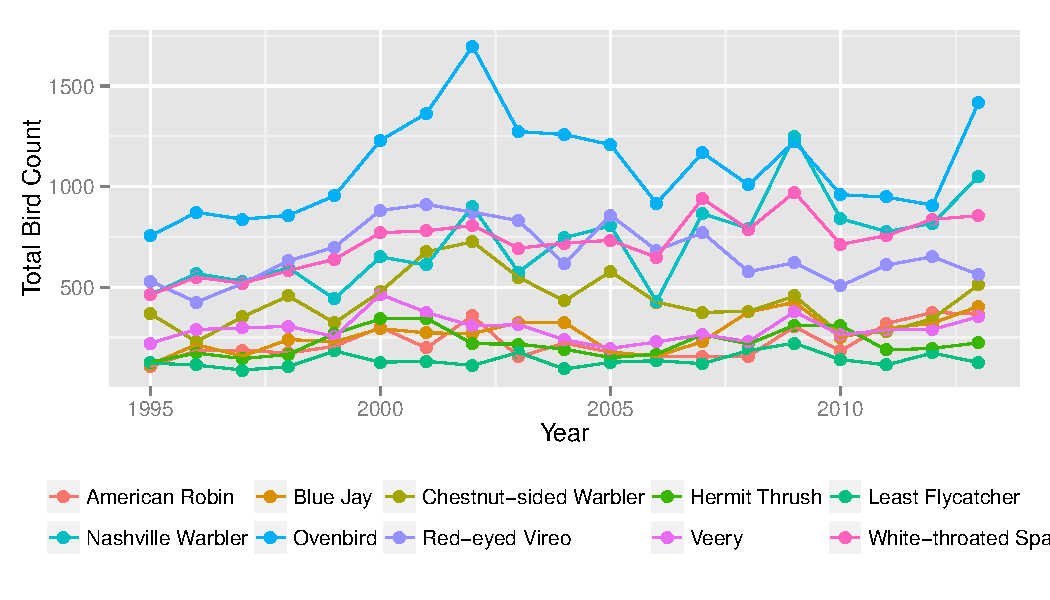
\includegraphics[width =\textwidth]{rawtrend}
%  \vspace{-.5in}
% \caption{Yearly total birds counts for the 10 selected species \label{figtr} \matt{Colors don't come through in black and white}}
% \end{figure}

Table \ref{tab:bird} provides summary statistics for the these data where total count is the actual number of birds counted within a year and mean count is the total count divided by the number of surveys, approximately 500 each year. The table then displays, for each species, the average and standard deviation of these total counts and mean counts across the years.

% latex table generated in R 3.0.2 by xtable 1.7-1 package
% Fri Aug 15 09:29:11 2014
\begin{table}[ht]
\centering
\caption{Summary statistics of bird count data in Superior National Forest from
1995 to 2013 for the 10 most abundant species.} 
\label{tab:bird}
\begin{tabular}{lcccc}
  \hline
  \multicolumn{1}{c}{Species} & \multicolumn{2}{c}{Total count} & \multicolumn{2}{c}{Mean count} \\
Name & Average & Stand. Dev. &Average & Stand. Dev.  \\ 
  \hline
Ovenbird & 1098 & 244 & 2.18 & 0.51 \\ 
  White-throated Sparrow & 725 & 135 & 1.43 & 0.24 \\ 
  Nashville Warbler & 722 & 214 & 1.42 & 0.36 \\ 
  Red-eyed Vireo & 672 & 145 & 1.34 & 0.33 \\ 
  Chestnut-sided Warbler & 432 & 133 & 0.86 & 0.28 \\ 
  Veery & 293 & 65 & 0.58 & 0.13 \\ 
  Blue Jay & 267 & 85 & 0.52 & 0.15 \\ 
  American Robin & 225 & 84 & 0.44 & 0.15 \\ 
  Hermit Thrush & 222 & 67 & 0.44 & 0.13 \\ 
  Least Flycatcher & 136 & 35 & 0.27 & 0.06 \\ 
   \hline
\end{tabular}
\end{table}

From a scientific perspective, the choice of whether to use the total count versus the mean count appears arbitrary when the purpose is to understand the correlation amongst species. But, due to our simulation results, we expect here that if we choose total count the correlation amongst the species will be well estimated. In contrast, if we choose mean count, the correlation will be biased toward zero and the estimated standard deviation will be biased toward larger values when using the IW prior. 

% The most abundant species, Ovenbirds , have around 1000 observations per year while the least abundant . The number of Ovenbirds seem to increase until 2002 when they reach the maximum count and decrease since that year, a similar pattern is suggested by the total counts in Chestnut−sided Warbler and Red−eyed Vireo so we expect these species to be positively correlated.  White−throated Sparrows and Nashville Warblers show an increasing pattern over the whole period, and the other species show a constant pattern.  
%Table \ref{count07} presents  mean and standard deviation  of the total bird count and the average count for each species, the species order in terms of abundance.  We can appreciate again the differences in total abundances among species, for intense, Ovenbirds are ten times more abundant than the Least Flycatcher. Recall we are selecting the ten most abundant species out of 73, which means there are species with really low counts in the entire counting season. 
%% latex table generated in R 3.0.2 by xtable 1.7-1 package
% Tue Apr  1 00:13:08 2014
\begin{table}[ht]
\centering
\caption{Total counts on 2007 for the 10 more abundant species} 
\begin{tabular}{llrrr}
  \hline
Specie & Abbrev & Chequamegon & Chippewa & Superior \\ 
  \hline
Least Flycatcher & OVEN & 1003 & 835 & 1168 \\ 
  Blue Jay & REVI & 823 & 997 & 771 \\ 
  White-throated Sparrow & NAWA & 240 & 348 & 867 \\ 
  Red-eyed Vireo & BLJA & 222 & 199 & 230 \\ 
  Nashville Warbler & CSWA & 211 & 330 & 375 \\ 
  Chestnut-sided Warbler & WTSP & 180 & 387 & 940 \\ 
  Ovenbird & HETH & 175 & 249 & 265 \\ 
  Veery & AMRO & 156 & 102 & 154 \\ 
  Hermit Thrush & LEFL & 155 & 368 & 120 \\ 
  American Robin & VEER &  91 & 402 & 264 \\ 
   \hline
\end{tabular}
\end{table}

%Also the information about the abbreviation for the species names is presented in Table \ref{count07} we won't use the common name of the species in the figures and pages that follow we use the abbreviation contained in this table. 
%As expected the sample variances for the total count are much higher than the variances of the mean. This give us the possibility of evaluate the effect of the scaling on the correlations inference, it is not clear that we should model the total count or the mean, so it would be possible to choose any of them. This arbitrary choice however may impact on the posterior inferences about the covariances matrix. 

\subsection{Correlation among Bird Species}

We run analyses of these data assuming a multivariate normal for each year with a mean of zero and an unknown covariance matrix. We assume the four prior distributions described in Table \ref{paramvals} as well as the IW prior using the scaled data. We also perform the analysis for each pair of species independently using a 2-dimensional normal and also simultaneously for all species using a 10-dimensional multivariate normal. Finally, we consider using the seemingly abitrary choice of total count and average count. 

These models are estimated with same methods used for the models with simulated data, using Stan software \citep{stan2014}. 

\begin{figure}[hbpt]
\centering
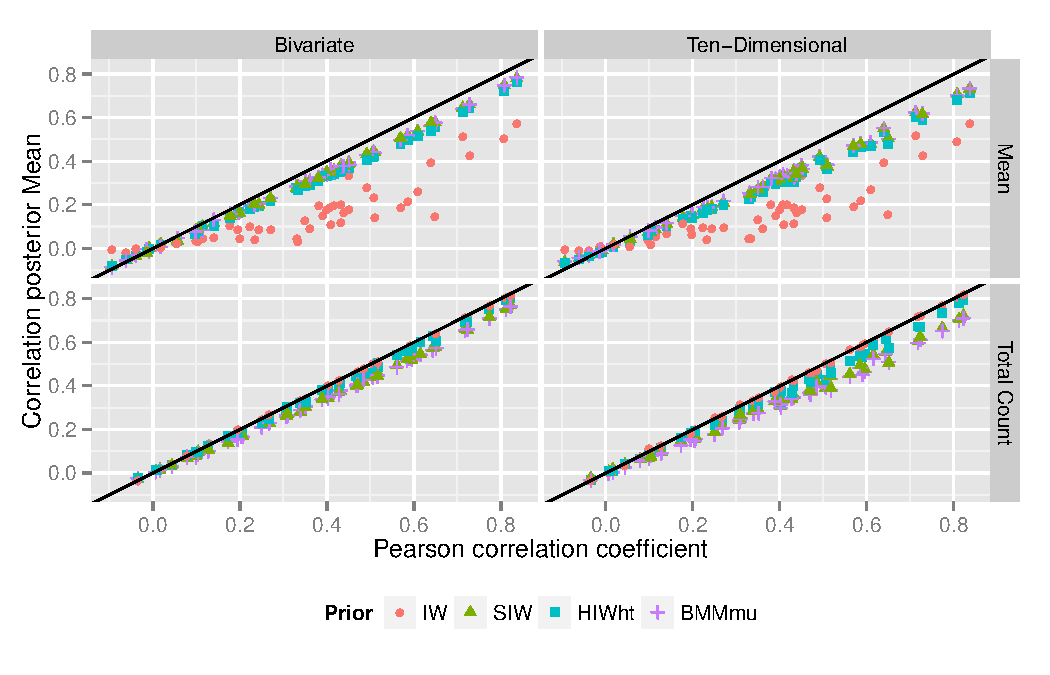
\includegraphics[width=\textwidth]{rescorr.pdf}
 \vspace{-.5in}
\caption{Posterior mean of the correlation for total count (bottom row) versus average count (top row) when performing the analysis for each pair of species independently (left column) versus all species simultaneously (right column) for four different priors on the covariance matrix as well as the IW prior using scaled data (IWsc).}
\label{fig:coring}
\end{figure}
%
%\begin{figure}[hbpt]
%\centering
%\includegraphics[width=\textwidth]{resvar}
% \vspace{-.5in}
%\caption{Standard deviation inference results. Scatter-plot of posterior mean for $\sigma_1$  against sample standard deviation. Only for ten dimensional case, columns panel represent response variable (average of the count or total count)  and color of the points represent the covariance prior. \label{birdsd}  }
%\end{figure}

Figure \ref{fig:coring} presents the estimated correlations. The posterior mean for each model is plotted against the Pearson correlation coefficient. The four panels represent each combination of response and dimension and within each panel there are four estimates for each pair of bird species corresponding to the five priors used. 

These results match those found when using simulated data. When we model mean count, we see each correlation estimate is shrunk towards zero, but the IW shrinkage is extreme. However the results change if we decide to model total count. Now there is no shrinkage towards small correlation values and, in fact, the IW prior may be the best at recovering the Pearson correlation coefficient.
%\matt{We were looking at posterior means before - why the sudden change to median? (FWIW I like the median better in all cases - for one we're certain it exists!)}

The SIW, HIW$_{ht}$ and BMM$_{mu}$ priors show similar behavior no matter which response is used to estimate the covariance matrix, and estimating correlation with any of these priors will lead to basically the same conclusions. 

%Inference about standard deviations is presented on figure \ref{birdsd}. Here we present only results for the ten dimensional models, the models using pairs of variables lead to several estimates for the same parameter because each species appears in nine different bivariate models. The standard deviation results also match what we found on simulated data, the only prior showing any problems is IW which overestimate (with respect to the sample standard deviation) standard deviations that are lower than 0.1. 
%\begin{figure}[hbpt]
%\centering
%\includegraphics[width=\textwidth]{corrmat}
% \vspace{-.5in}
%\caption{Correlation matrix among ten species used in the study. Using BMM$_{mu}$ prior, average count, and ten dimensional model \label{fig:mat}}
%\end{figure}
%Figure \ref{fig:mat} present the estimated correlation matrix using an BMM$_{mu}$ prior, on a ten dimensional model and an average count as a response. There were no negative correlated species among the most abundant ones. We can see there are some species forming a sort of a 'cluster" in the series that all are highly correlated, as  OVEN, REVI and CSWA (maybe WTSP could be in this group too).  On the other hand there are a couple of species which shows small correlations with all the rest, this is specially true for LEFL and also AMRO.  
%\begin{figure}[hbpt]
%\centering
%\includegraphics[width=\textwidth]{spcor}
% \vspace{-.5in}
%\caption{Trend in some selected species. OVEN, REVI and CSWA are highly correlated while LEFL and AMRO shows no correlation with other species. \label{trend}}
%\end{figure}
%Figure \ref{trend}  shows the dynamics for the five species identify on the correlation matrix. AS the data are centered, the lines represent the difference between the average yearly count and the historical mean for that species. The three species with high correlation shows the same temporal pattern, a sort of inverted u-shape specially marked on the case of OVEN. The two species with small correlation have a very stable pattern with no big departures from its own mean. 

\subsection{Hierarchical linear model} 
A posible hierarchical model in this scenario is 
\[\begin{array}{ccc}
y_{st} \sim N(x_t^{\top}\beta_s,\; \sigma^2) & & \beta_s \sim N(0, \Sigma)
\end{array}
\]
where $x_t^{\top} = (1,\; t,\; t^2)$. In order to have full Bayesian inference in this model we might set independent priors for the variances $\Sigma\sim IW(I, d+1)$ and $\sigma \sim Cauchy^{+}(0,1)$. 

\begin{figure}[htbp]
\centering
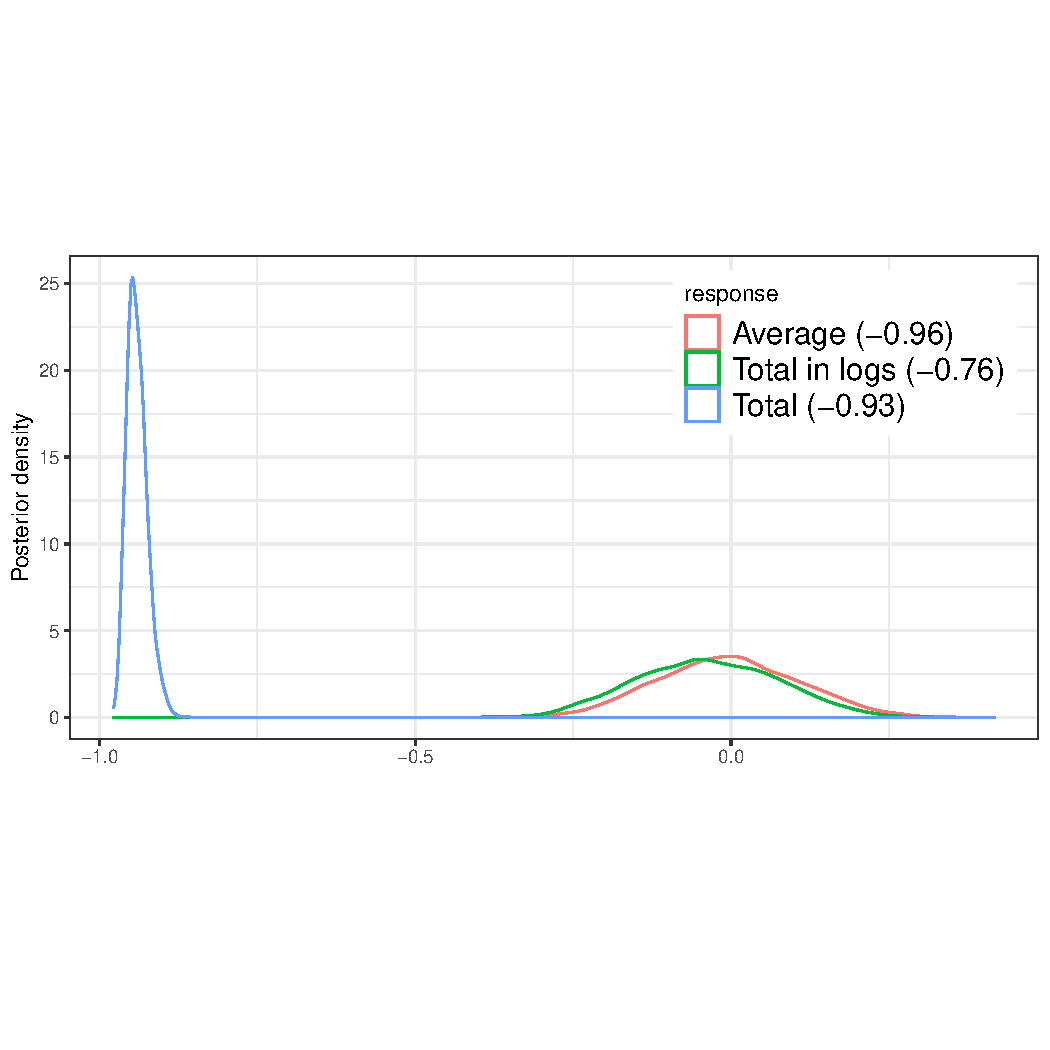
\includegraphics[trim = 0 4cm 0 3cm, clip, scale=.5]{reg_3modIW.pdf} 
%\vspace{-.5in}
\caption{ posterior of correlation between coeficients }
\label{linear} 
\end{figure}


\section{Summary \label{sec:summary}} 

Simulations from the IW prior show a strong \emph{a priori} dependence between the correlation and the variances. The SIW and HIW$_{ht}$ priors show a similar dependence but both seem to be more flexible than the IW prior. The BMM$_{mu}$ prior presents the most flexibility since variances and correlations are independent by construction.

Posterior results for the IW prior show an extreme bias toward larger values for small empirical variances and a corresponding shrinkage of the estimated correlation toward zero. In contrast, the other three priors show only a slight bias toward zero correlations and this is attenuated completely for larger sample sizes.

From a modeling perspective, the BMM$_{mu}$ prior flexibility is appealing since we can model correlations and variances independently and let the data define their relationship.  The BMM$_{mu}$ prior is the original proposal of \cite{barnard2000}, however a separation strategy could use a different prior for variances and correlations, e.g. a half-t for the standard deviations and uniform for the correlations. 

From a computational perspective we expect the BMM$_{mu}$ prior to be the most complex, since all the others conserve the conjugacy properties of the IW distribution. This is especially relevant for a Gibbs sampler, where conjugacy allows for a Gibbs steps. Using Stan or any other HMC-based approach, there is relatively little cost to using other prior such as BMM$_{mu}$. 
Computationally, the SIW prior is more efficient than HIW or BMM even when using Stan \citep{CCalvarez}. 

In summary, the prior choice may depend on which are the computational resources are available. If it is possible to use a HMC sampler such as STAN, the separation strategy proposed by \cite{barnard2000} gives modeling flexibility and good inference properties. Whenever we use Gibbs based samplers, e.g. JAGS or BUGS, a prior which maintains some conjugacy might be preferable. For some Bayesian software, the IW prior may be our only option. In this case, if our only objective is to estimate the correlation, it is possible to pre-scale that data such that each component as an empirical variance of 1 and then proceed with the IW prior. This appears to provide unbiased estimates of the correlations \citep{CCalvarez}. 
% There are multiple ways in which we could continue with this line of work. However, there are three issues that seems more natural ways to continue.  \matt{This part seems both a bit out of place and lacking some detail. Probably you just need a better transition into it and to discuss it in paragraph form.} 
%\begin{description}
%\item[Different Model] Extend the simulation analysis to a hierarchical linear model context, since the effect of $p(\Sigma)$ might be different \citep{gelman2006prior}. 
%\item[Different Scenarios]  Use different true covariance structures. 
%\item[Different Priors] For instance, use $LKJ$ prior for the correlation matrix or use other distributions for IW parameters $\nu$ and $\Lambda$.
%\end{description}

\bibliographystyle{asa}      
\bibliography{report_year}      
\end{document}